%--------------------------------------------------
\section{Study of QCD shape and normalization in MC}
Since there are not enough QCD events passing all of the cuts, we relax some of them. Specifically, the new requirements are
\begin{itemize}
\item MET$>20.0$~GeV for both muons and electrons.
\item Isolation$>0.3$ for both muons and electrons.
\item $WP80$ restrictions are removed for electrons.
\end{itemize}
This approach does not alter the shapes of the W transverse mass distributions
(Figure~\ref{fig:QCDCutLoosening}) and provides a sufficient number of
events (300-500) to construct the templates. Furthermore, since the
W transverse mass distribution should be the same for all processes except
QCD, we perform a fit to the data using the W$jj$, QCD templates -
Figure~\ref{fig:QCDTemplateFit} and fix the fraction of QCD relative
to W$jj$. After accounting for acceptances of the above cuts these
are: $\mu$ $frac_{QCD}=0.0053\pm 0.00050$, $el$ $frac_{QCD}=0.0386\pm
0.00486$.

%%%%%%%%%%%%%%%%%%%%%%%%%%%%
%%%%%%%
\begin{figure}[h!] {\centering
\unitlength=0.33\linewidth
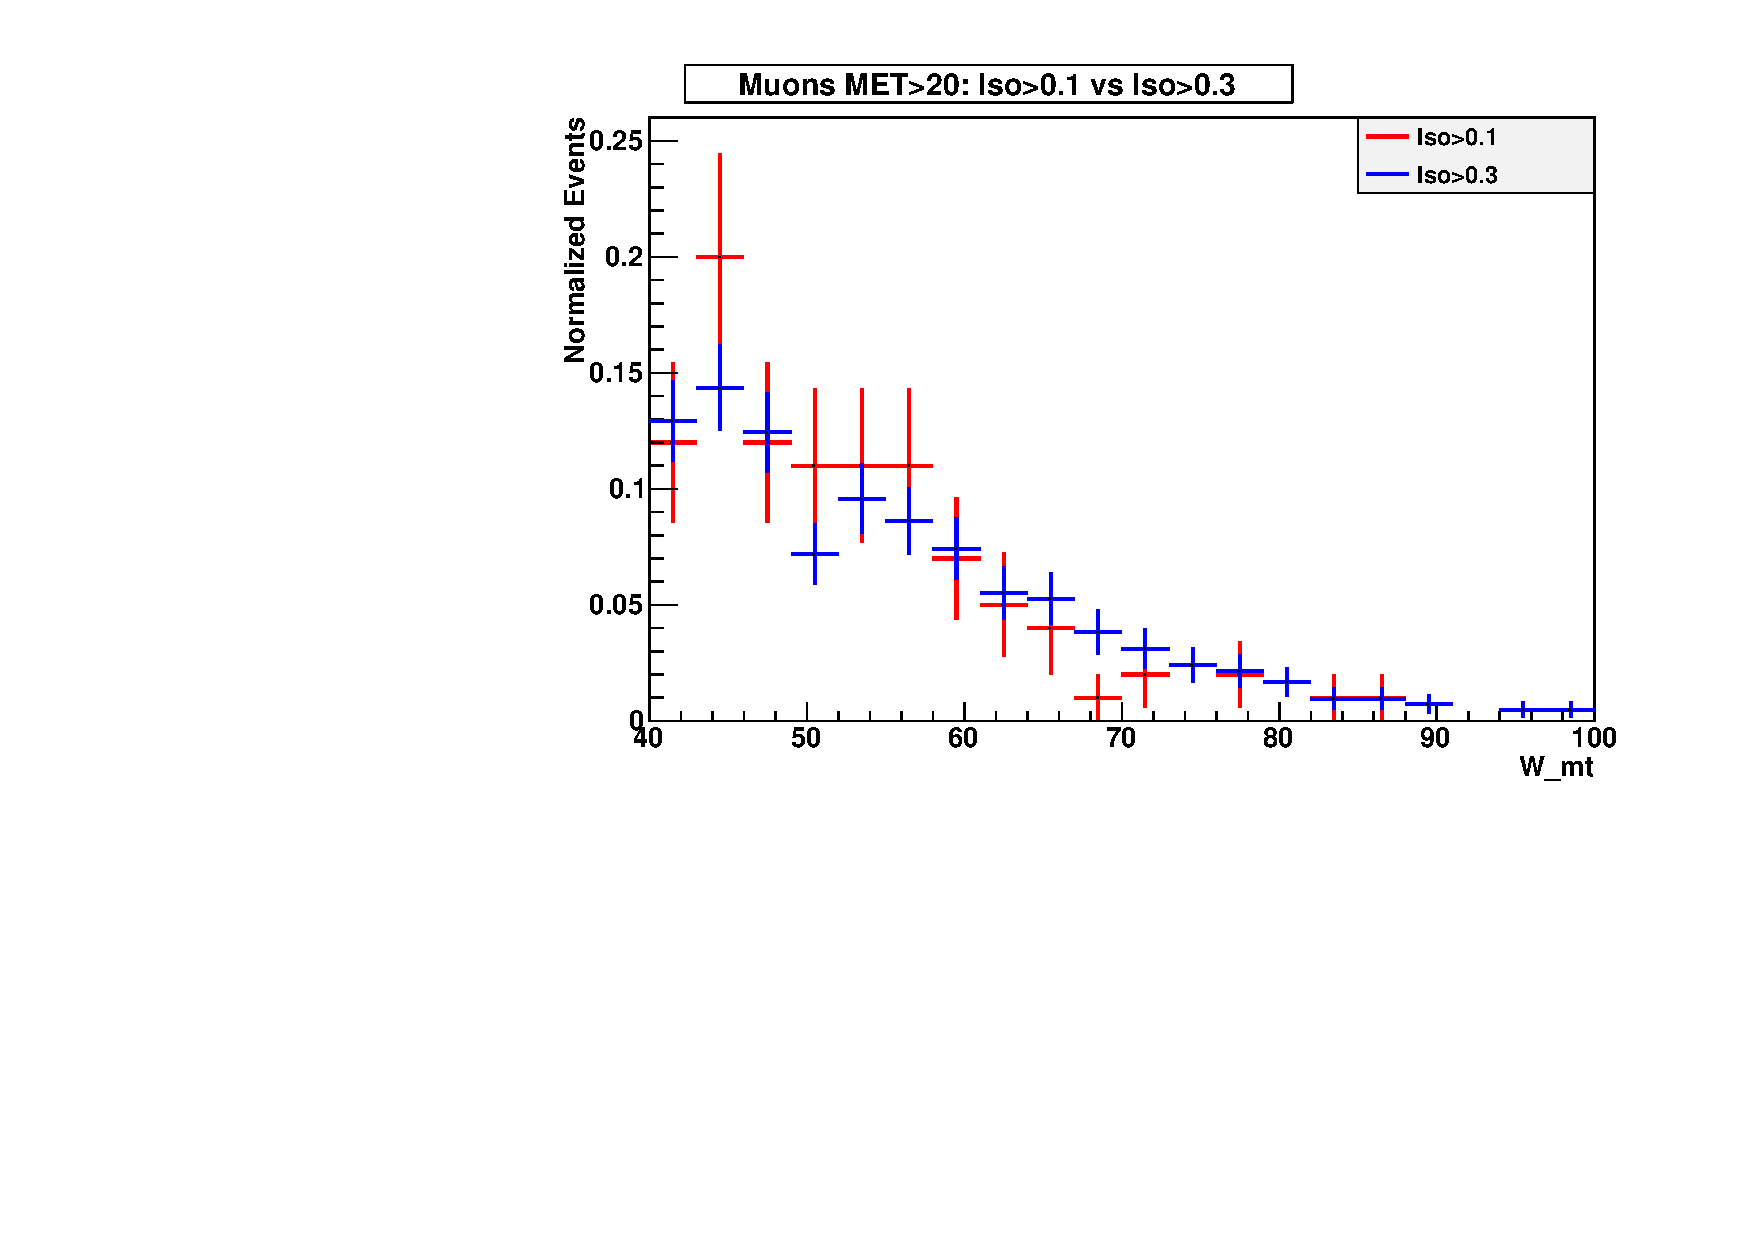
\includegraphics[width=0.48\textwidth]{figs/QCDCutLoosening_mu.pdf}
\put(-0.80,0.0){(a)} 
\unitlength=0.33\linewidth
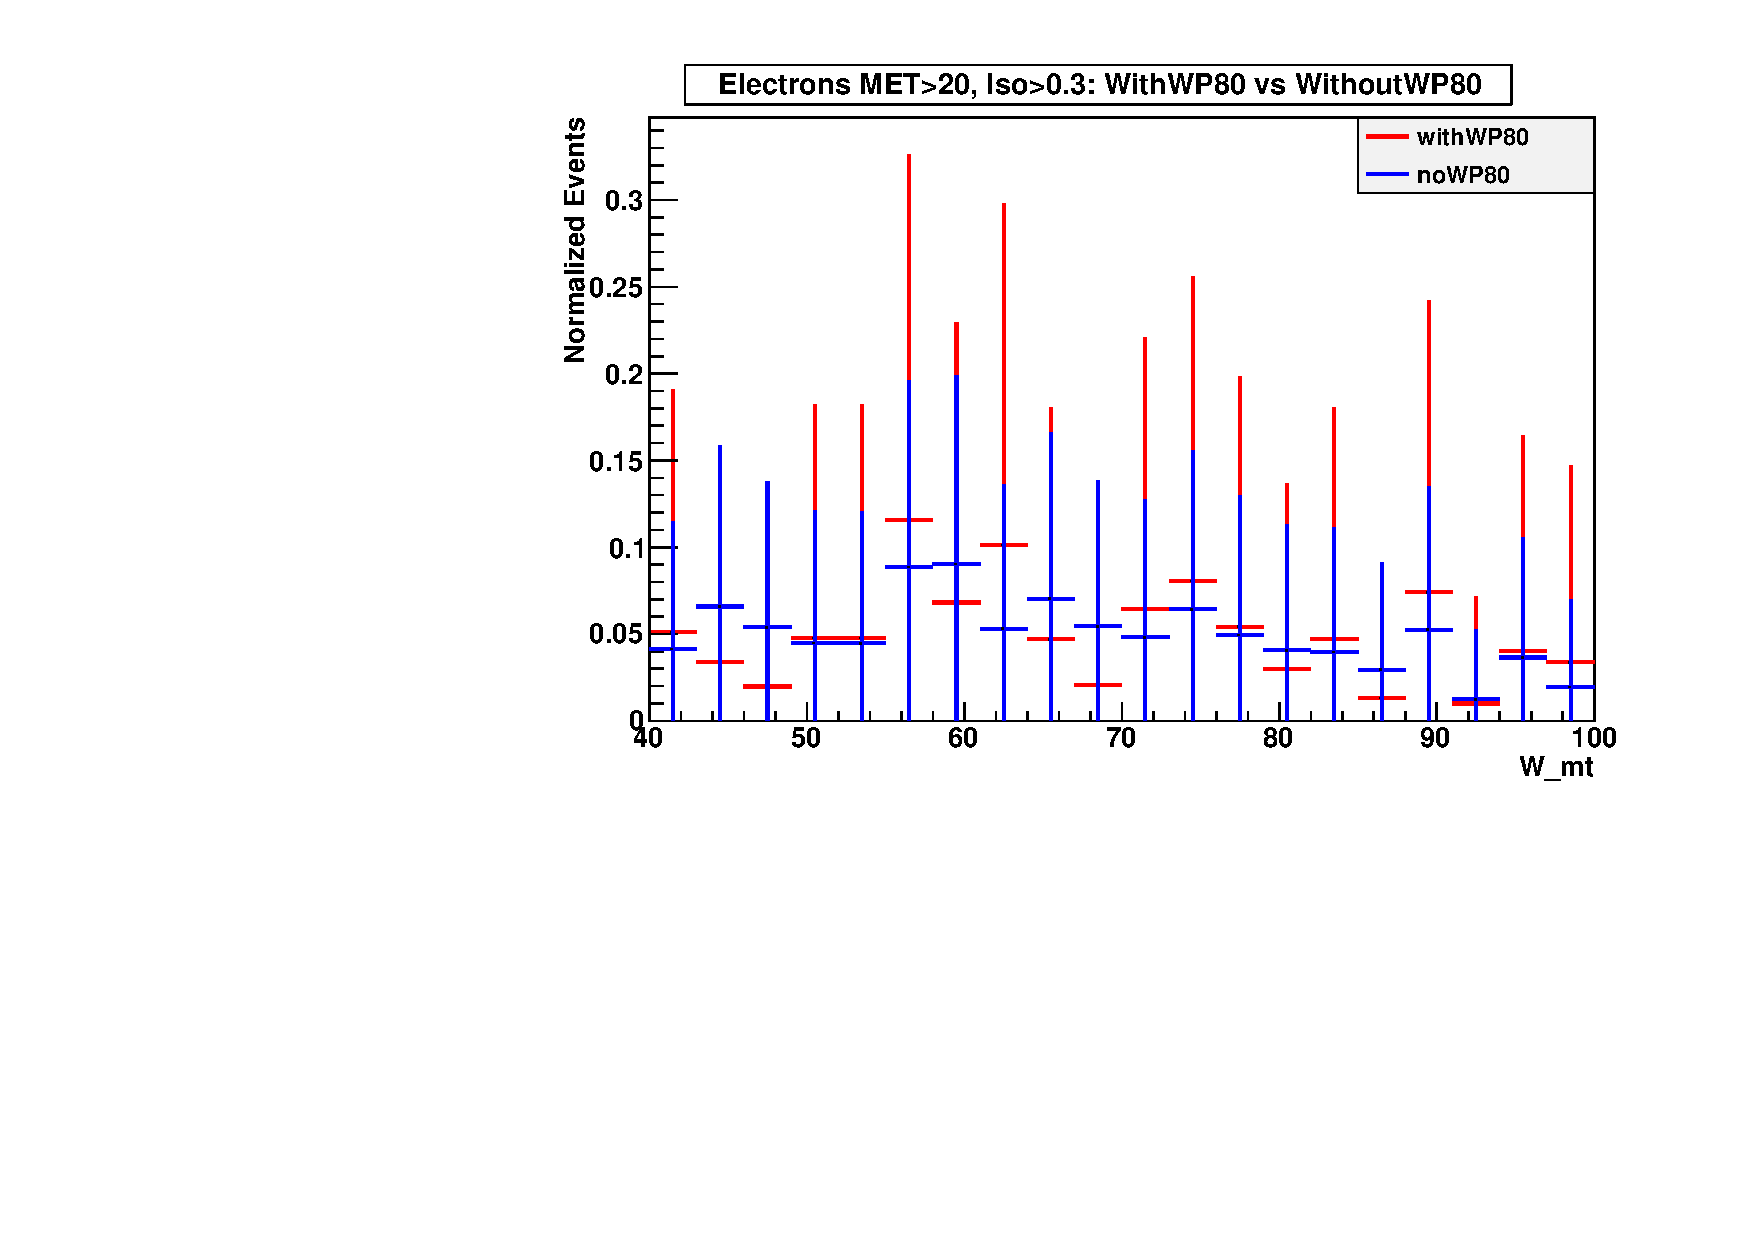
\includegraphics[width=0.48\textwidth]{figs/QCDCutLoosening_el.pdf}
\put(-0.80,0.0){(b)} 
\caption{ Comparison of the $W_{mT}$ shapes before and after loosening the (MET, Isolation and $WP80$) cuts for (a) muon QCD, (b) electron QCD distribution. The two are statistically consistent.} 
\label{fig:QCDCutLoosening}}
\end{figure}
%%%%%%%
%%%%%%%
\begin{figure}[h!] {\centering
\unitlength=0.33\linewidth
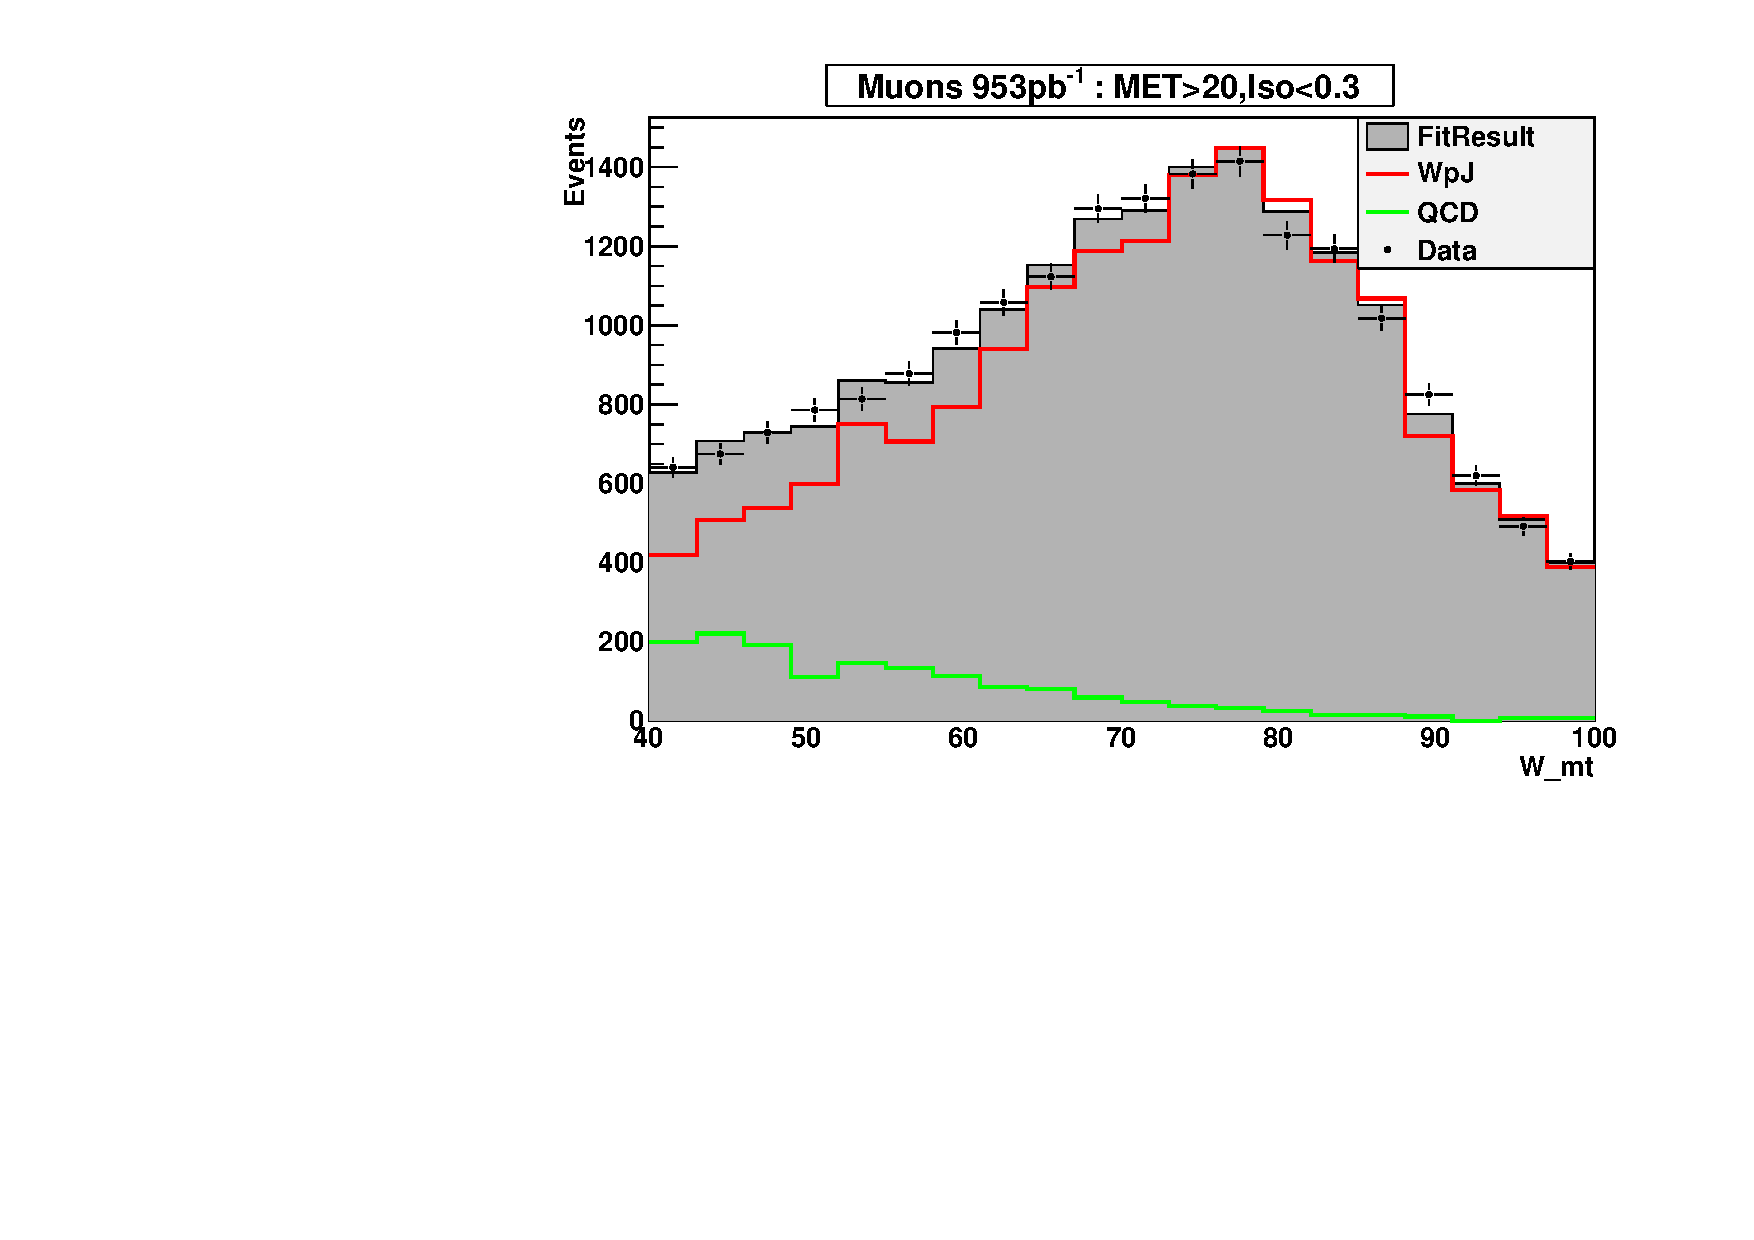
\includegraphics[width=0.48\textwidth]{figs/QCDTemplateFit_mu.pdf}
\put(-0.80,0.0){(a)} 
\unitlength=0.33\linewidth
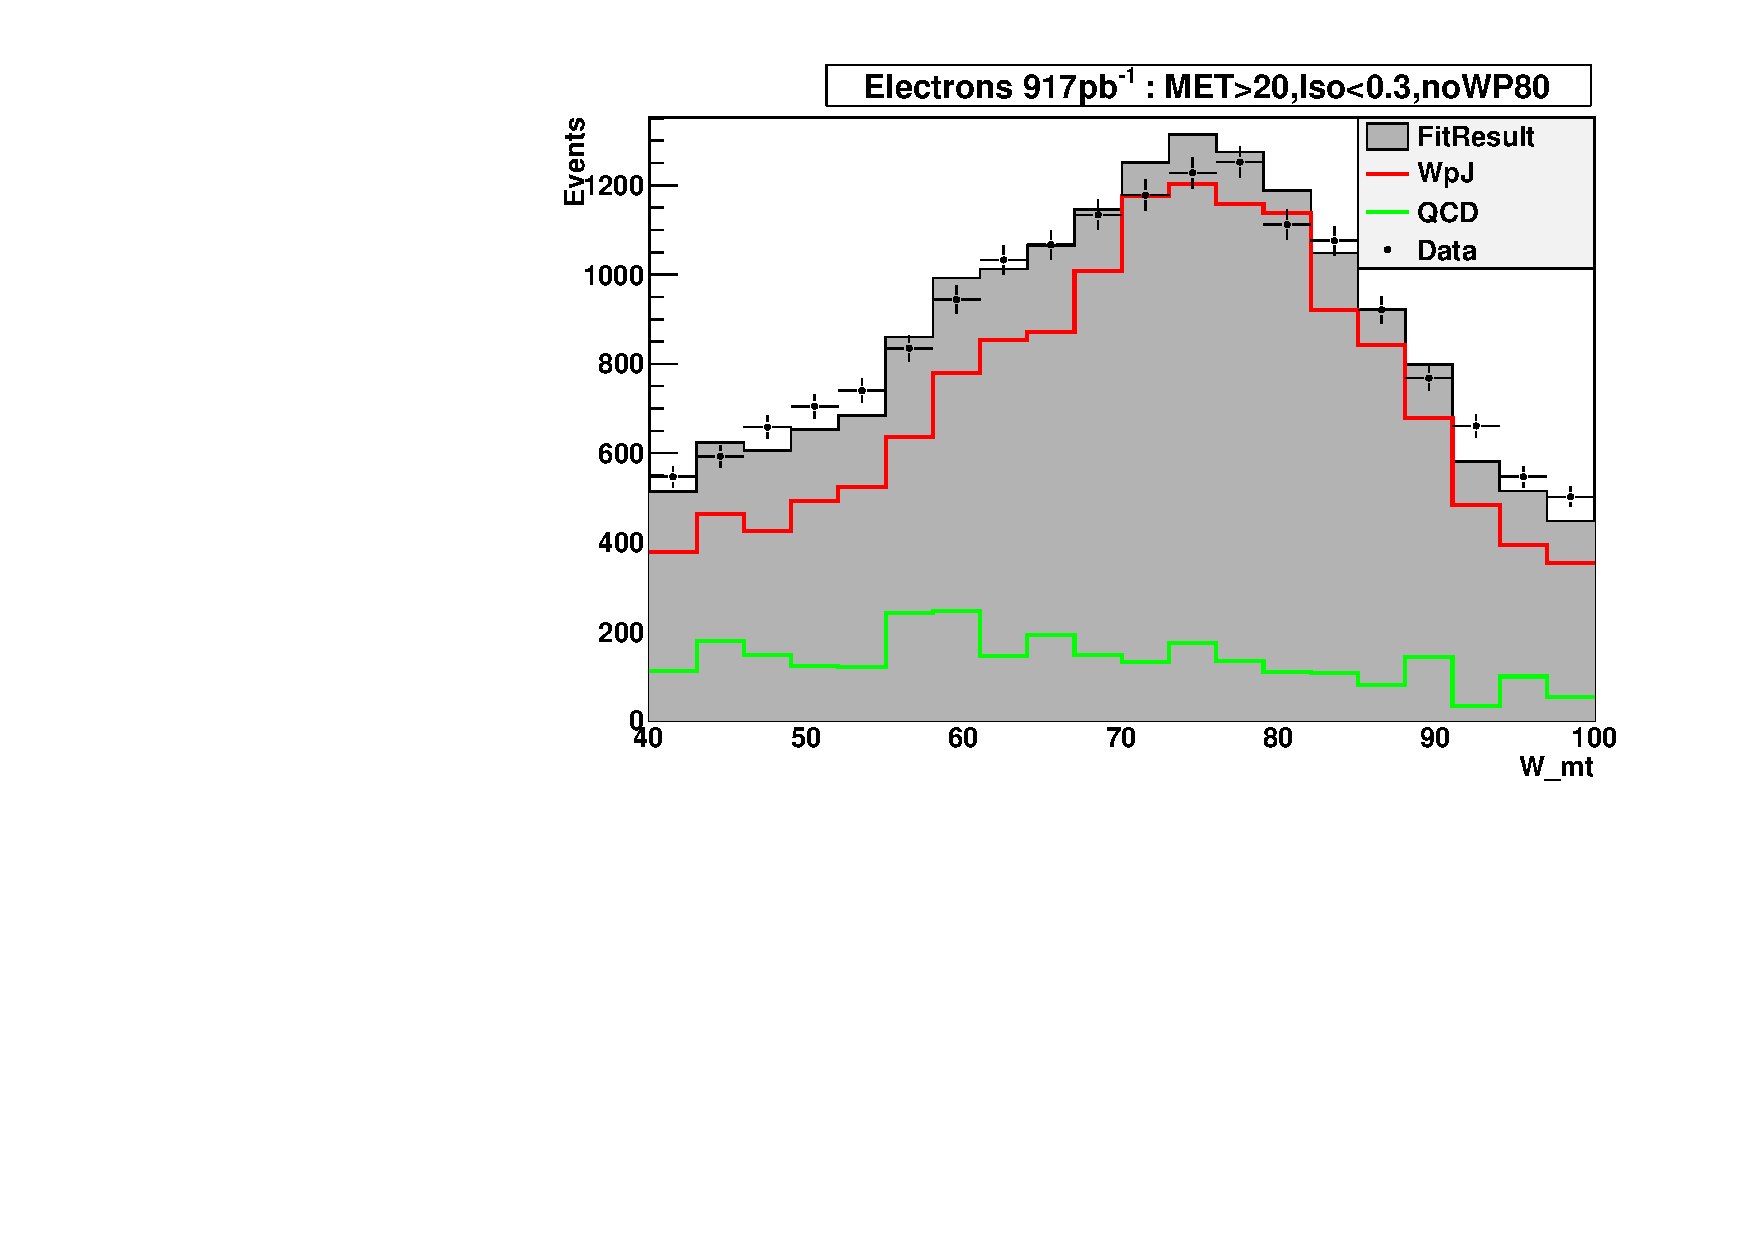
\includegraphics[width=0.48\textwidth]{figs/QCDTemplateFit_el.pdf}
\put(-0.80,0.0){(b)} 
\caption{$W_{mT}$ fit using QCD and W$jj$ templates for (a) muon, (b) electron data.} 
\label{fig:QCDTemplateFit}}
\end{figure}
%%%%%%%
